% Experimental Evaluation
% 子图标签样式：显示为 (a) (b)
\captionsetup[subfigure]{labelformat=parens,labelsep=space}
\begin{table}[t]
%   \tiny
  \centering
  \caption{Statistics of Datasets.}
  \label{tab:graph-stats}
  \setlength{\tabcolsep}{3pt}
  {\color{black}\arrayrulecolor{black}%
  \begin{tabular}{@{\hspace{3pt}}c@{\hspace{3pt}}c@{\hspace{3pt}}c@{\hspace{3pt}}c@{\hspace{3pt}}c@{\hspace{3pt}}c@{\hspace{3pt}}c@{\hspace{3pt}}}
    \toprule
    Dataset     & {$n$}       & {$m$}        & {$\mathrm{Avg\ deg.}$} & {$\mathrm{Max\ deg.}$} & {\#Triangles} & {$\mathrm{Max\ Clique}$} \\
    \midrule
    com-dblp(DBLP)        & 317\,081     & 1\,049\,867   & 6.6   & 343      & 2\,224\,385    & 114 \\
    web-Stanford(STF)    & 281\,903     & 1\,992\,636   & 14.1  & 38\,625  & 11\,329\,473   & 61 \\
    com-youtube(YT)     & 1\,134\,890  & 2\,987\,624   & 5.3   & 28\,754  & 3\,056\,386    & 17 \\
    web-Google(GO)      & 875\,713     & 4\,322\,051   & 9.9   & 6\,332   & 13\,391\,903   & 44 \\
    web-it-2004(WI)     & 509\,338     & 7\,178\,413   & 28.2  & 469      & 338\,884\,212  & 432 \\
    soc-pokec(PO)       & 1\,632\,803  & 22\,301\,964  & 27.3  & 14\,854  & 32\,557\,458   & 29 \\
    \bottomrule
  \end{tabular}}
\end{table}


\afterpage{
\begin{figure*}
  \centering
    \captionsetup[subfigure]{font=tiny, skip=0pt}
  
  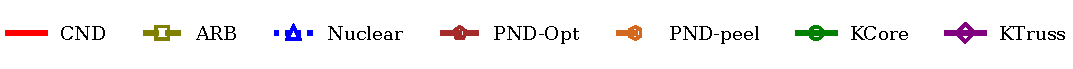
\includegraphics[width=0.9\linewidth]{figure/legend_algorithms_fixed_lines.pdf}

    \begin{minipage}[c]{0.02\textwidth}
    \centering
    \raisebox{2em}{\rotatebox{90}{\tiny \textbf{Time(s)}}} 
  \end{minipage}  \begin{subfigure}[t]{0.158\textwidth}
    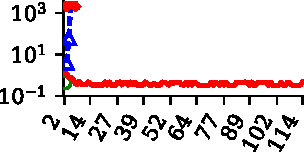
\includegraphics[width=\linewidth]{figure/com-dblp_r1_time_by_s_No_Hi.pdf}
    \caption{\myaddRA{DBLP$s\{r{=}1\}$}}
  \end{subfigure}\hfill
  \begin{subfigure}[t]{0.158\textwidth}
    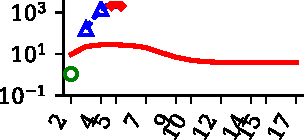
\includegraphics[width=\linewidth]{figure/com-youtube_r1_time_by_s_No_Hi.pdf}
    \caption{YT $s\{r{=}1\}$}
  \end{subfigure}\hfill
  \begin{subfigure}[t]{0.158\textwidth}
    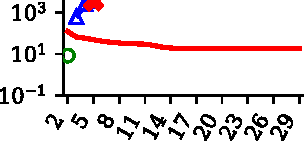
\includegraphics[width=\linewidth]{figure/soc-pokec-relationships_r1_time_by_s_No_Hi.pdf}
    \caption{PO $s\{r{=}1\}$}
  \end{subfigure}\hfill
  \begin{subfigure}[t]{0.158\textwidth}
    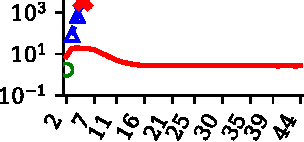
\includegraphics[width=\linewidth]{figure/web-Google_r1_time_by_s_No_Hi.pdf}
    \caption{GO $s\{r{=}1\}$}
  \end{subfigure}\hfill
  \begin{subfigure}[t]{0.158\textwidth}
    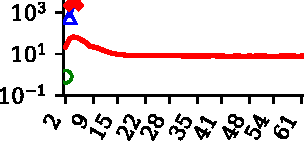
\includegraphics[width=\linewidth]{figure/web-Stanford_r1_time_by_s_No_Hi.pdf}
    \caption{STF $s\{r{=}1\}$}
  \end{subfigure}\hfill
  \begin{subfigure}[t]{0.158\textwidth}
    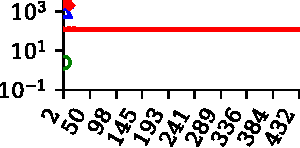
\includegraphics[width=\linewidth]{figure/web-it-2004_r1_time_by_s_No_Hi.pdf}
    \caption{WI $s\{r{=}1\}$}
  \end{subfigure}
  
  

    \begin{minipage}[c]{0.02\textwidth}
    \centering
    \raisebox{2em}{\rotatebox{90}{\tiny \textbf{Time(s)}}} 
  \end{minipage}  \begin{subfigure}[t]{0.158\textwidth}
    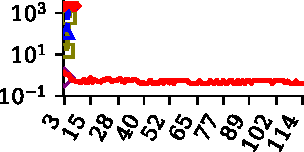
\includegraphics[width=\linewidth]{figure/com-dblp_r2_time_by_s_No_Hi.pdf}
    \caption{\myaddRA{DBLP$s\{r{=}2\}$}}
  \end{subfigure}\hfill
  \begin{subfigure}[t]{0.158\textwidth}
    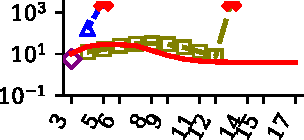
\includegraphics[width=\linewidth]{figure/com-youtube_r2_time_by_s_No_Hi.pdf}
    \caption{YT $s\{r{=}2\}$}
    \label{fig:youtube_r2_time_by_s}
  \end{subfigure}\hfill
  \begin{subfigure}[t]{0.158\textwidth}
    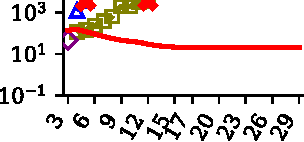
\includegraphics[width=\linewidth]{figure/soc-pokec-relationships_r2_time_by_s_No_Hi.pdf}
    \caption{PO $s\{r{=}2\}$}
  \end{subfigure}\hfill
  \begin{subfigure}[t]{0.158\textwidth}
    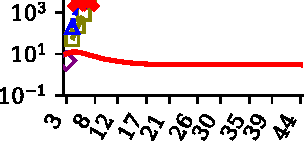
\includegraphics[width=\linewidth]{figure/web-Google_r2_time_by_s_No_Hi.pdf}
    \caption{GO $s\{r{=}2\}$}
  \end{subfigure}\hfill
  \begin{subfigure}[t]{0.158\textwidth}
    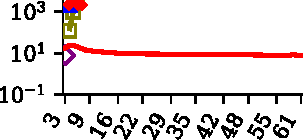
\includegraphics[width=\linewidth]{figure/web-Stanford_r2_time_by_s_No_Hi.pdf}
    \caption{STF $s\{r{=}2\}$}
  \end{subfigure}\hfill
  \begin{subfigure}[t]{0.158\textwidth}
    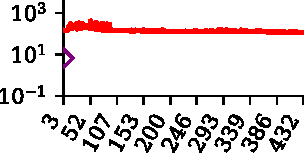
\includegraphics[width=\linewidth]{figure/web-it-2004_r2_time_by_s_No_Hi.pdf}
    \caption{WI $s\{r{=}2\}$}
  \end{subfigure}

  
  \caption{Running time (seconds) across $s$ without hierarchy for $r = 1$(a-f) and $r=2$(g-l).}
  \label{fig:r1r2_time_by_s}

  
    \begin{minipage}[c]{0.02\textwidth}
    \centering
    \raisebox{2em}{\rotatebox{90}{\tiny \textbf{Time(s)}}} 
  \end{minipage}  \begin{subfigure}[t]{0.158\textwidth}
    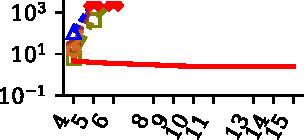
\includegraphics[width=\linewidth]{figure/com-dblp_r3_time_by_s_No_Hi.pdf}
    \caption{\myaddRA{DBLP$s\{r{=}3\}$}}
  \end{subfigure}\hfill
  \begin{subfigure}[t]{0.158\textwidth}
    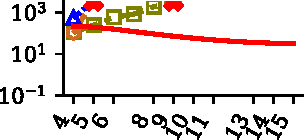
\includegraphics[width=\linewidth]{figure/soc-pokec-relationships_r3_time_by_s_No_Hi.pdf}
    \caption{PO $s\{r{=}3\}$}
  \end{subfigure}\hfill
  \begin{subfigure}[t]{0.158\textwidth}
    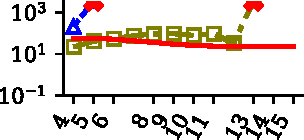
\includegraphics[width=\linewidth]{figure/com-youtube_r3_time_by_s_No_Hi.pdf}
    \caption{YT $s\{r{=}3\}$}
  \end{subfigure}\hfill
  \begin{subfigure}[t]{0.158\textwidth}
    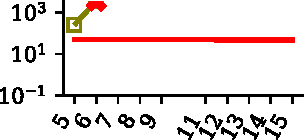
\includegraphics[width=\linewidth]{figure/com-dblp_r4_time_by_s_No_Hi.pdf}
    \caption{DBLP $s\{r{=}4\}$}
  \end{subfigure}\hfill
  \begin{subfigure}[t]{0.158\textwidth}
    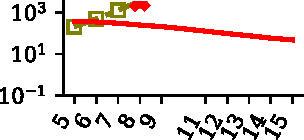
\includegraphics[width=\linewidth]{figure/soc-pokec-relationships_r4_time_by_s_No_Hi.pdf}
    \caption{PO $s\{r{=}4\}$}
  \end{subfigure}\hfill
  \begin{subfigure}[t]{0.158\textwidth}
    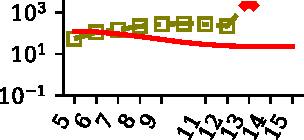
\includegraphics[width=\linewidth]{figure/com-youtube_r4_time_by_s_No_Hi.pdf}
    \caption{YT $s\{r{=}4\}$}
  \end{subfigure}

  

    \begin{minipage}[c]{0.02\textwidth}
    \centering
    \raisebox{2em}{\rotatebox{90}{\tiny \textbf{Time(s)}}} 
  \end{minipage}  \begin{subfigure}[t]{0.158\textwidth}
    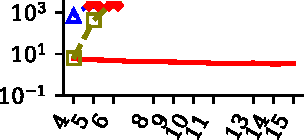
\includegraphics[width=\linewidth]{figure/com-dblp_r3_time_by_s.pdf}
    \caption{DBLP $s\{r{=}3\}$}
  \end{subfigure}\hfill
  \begin{subfigure}[t]{0.158\textwidth}
    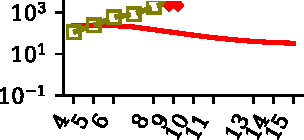
\includegraphics[width=\linewidth]{figure/soc-pokec-relationships_r3_time_by_s.pdf}
    \caption{PO $s\{r{=}3\}$}
  \end{subfigure}\hfill
  \begin{subfigure}[t]{0.158\textwidth}
    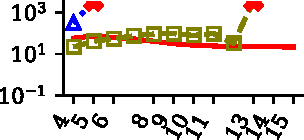
\includegraphics[width=\linewidth]{figure/com-youtube_r3_time_by_s.pdf}
    \caption{YT $s\{r{=}3\}$}
  \end{subfigure}\hfill
  \begin{subfigure}[t]{0.158\textwidth}
    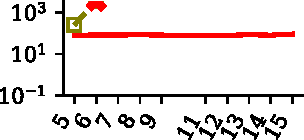
\includegraphics[width=\linewidth]{figure/com-dblp_r4_time_by_s.pdf}
    \caption{DBLP $s\{r{=}4\}$}
  \end{subfigure}\hfill
  \begin{subfigure}[t]{0.158\textwidth}
    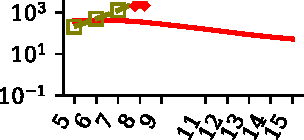
\includegraphics[width=\linewidth]{figure/soc-pokec-relationships_r4_time_by_s.pdf}
    \caption{PO $s\{r{=}4\}$}
  \end{subfigure}\hfill
  \begin{subfigure}[t]{0.158\textwidth}
    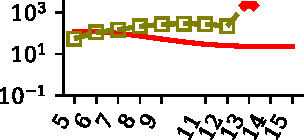
\includegraphics[width=\linewidth]{figure/com-youtube_r4_time_by_s.pdf}
    \caption{YT $s\{r{=}4\}$}
  \end{subfigure}

  
  \caption{Running time (seconds) across $s$ for $r \in \{3,4\}$(a-f without hierarchy; g-l with hierarchy).}
  \label{fig:time_by_s_r3_r4_combined}

  
    \begin{minipage}[c]{0.02\textwidth}
    \centering
    \raisebox{2em}{\rotatebox{90}{\tiny \textbf{Time(s)}}} 
  \end{minipage}  \begin{subfigure}[t]{0.158\textwidth}
      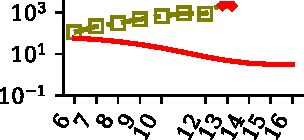
\includegraphics[width=\linewidth]{figure/com-youtube_r5_time_by_s_No_Hi.pdf}
      \caption{YT $s\{r{=}5\}$}
  \end{subfigure}\hfill
  \begin{subfigure}[t]{0.158\textwidth}
      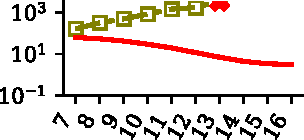
\includegraphics[width=\linewidth]{figure/com-youtube_r6_time_by_s_No_Hi.pdf}
      \caption{YT $s\{r{=}6\}$}
  \end{subfigure}\hfill
  \begin{subfigure}[t]{0.158\textwidth}
      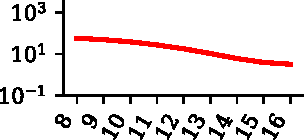
\includegraphics[width=\linewidth]{figure/com-youtube_r7_time_by_s_No_Hi.pdf}
      \caption{YT $s\{r{=}7\}$}
  \end{subfigure}\hfill
  \begin{subfigure}[t]{0.158\textwidth}
      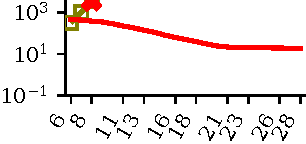
\includegraphics[width=\linewidth]{figure/soc-pokec-relationships_r5_time_by_s_no_hi-eps-converted-to.pdf}
      \caption{PO $s\{r{=}5\}$}
  \end{subfigure}\hfill
  \begin{subfigure}[t]{0.158\textwidth}
      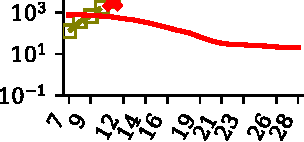
\includegraphics[width=\linewidth]{figure/soc-pokec-relationships_r6_time_by_s_no_hi.pdf}
      \caption{PO $s\{r{=}6\}$}
  \end{subfigure}\hfill
  \begin{subfigure}[t]{0.158\textwidth}
      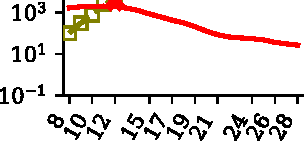
\includegraphics[width=\linewidth]{figure/soc-pokec-relationships_r7_time_by_s_no_hi.pdf}
      \caption{PO $s\{r{=}7\}$}
  \end{subfigure}

  
  \caption{Running time (seconds) across $s$ without hierarchy for $r \in \{5,6,7\}$.}
  \label{fig:time_by_s_r5_r7_combined}

    \begin{minipage}[c]{0.02\textwidth}
    \centering
    \raisebox{3em}{\rotatebox{90}{\tiny \textbf{Mem(MB)}}} 
  \end{minipage}  \begin{subfigure}[t]{0.158\textwidth}
    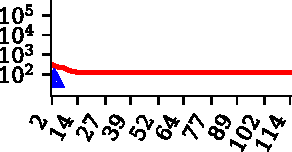
\includegraphics[width=\linewidth]{figure/com-dblp_r1_memory_by_s_no_hi.pdf}
    \caption{DBLP $s\{r{=}1\}$}
  \end{subfigure}\hfill
  \begin{subfigure}[t]{0.158\textwidth}
    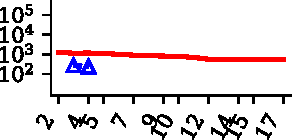
\includegraphics[width=\linewidth]{figure/com-youtube_r1_memory_by_s_no_hi.pdf}
    \caption{YT $s\{r{=}1\}$}
  \end{subfigure}\hfill
  \begin{subfigure}[t]{0.158\textwidth}
    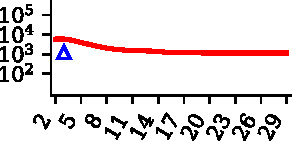
\includegraphics[width=\linewidth]{figure/soc-pokec-relationships_r1_memory_by_s_no_hi.pdf}
    \caption{PO $s\{r{=}1\}$}
  \end{subfigure}\hfill
  \begin{subfigure}[t]{0.158\textwidth}
    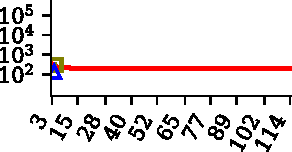
\includegraphics[width=\linewidth]{figure/com-dblp_r2_memory_by_s_no_hi.pdf}
    \caption{DBLP $s\{r{=}2\}$}
  \end{subfigure}\hfill
  \begin{subfigure}[t]{0.158\textwidth}
    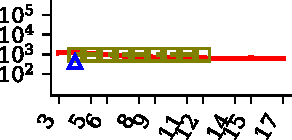
\includegraphics[width=\linewidth]{figure/com-youtube_r2_memory_by_s_no_hi.pdf}
    \caption{YT $s\{r{=}2\}$}
  \end{subfigure}\hfill
  \begin{subfigure}[t]{0.158\textwidth}
    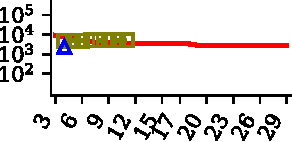
\includegraphics[width=\linewidth]{figure/soc-pokec-relationships_r2_memory_by_s_no_hi.pdf}
    \caption{PO $s\{r{=}2\}$}
  \end{subfigure}

    \begin{minipage}[c]{0.02\textwidth}
    \centering
    \raisebox{3em}{\rotatebox{90}{\tiny \textbf{Mem(MB)}}}
  \end{minipage}  
  \begin{subfigure}[t]{0.158\textwidth}
    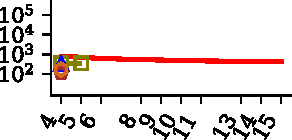
\includegraphics[width=\linewidth]{figure/com-dblp_r3_memory_by_s_no_hi.pdf}
    \caption{DBLP $s\{r{=}3\}$}
  \end{subfigure}\hfill
  \begin{subfigure}[t]{0.158\textwidth}
    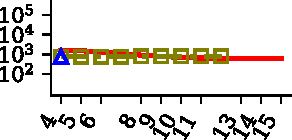
\includegraphics[width=\linewidth]{figure/com-youtube_r3_memory_by_s_no_hi.pdf}
    \caption{YT $s\{r{=}3\}$}
  \end{subfigure}\hfill
  \begin{subfigure}[t]{0.158\textwidth}
    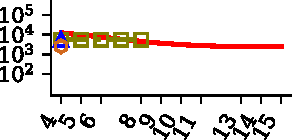
\includegraphics[width=\linewidth]{figure/soc-pokec-relationships_r3_memory_by_s_no_hi.pdf}
    \caption{PO $s\{r{=}3\}$}
  \end{subfigure}\hfill
  \begin{subfigure}[t]{0.158\textwidth}
    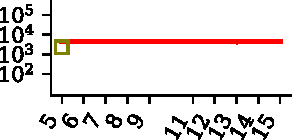
\includegraphics[width=\linewidth]{figure/com-dblp_r4_memory_by_s_no_hi.pdf}
    \caption{DBLP $s\{r{=}4\}$}
  \end{subfigure}\hfill
  \begin{subfigure}[t]{0.158\textwidth}
    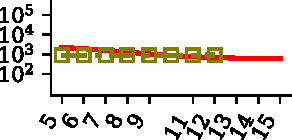
\includegraphics[width=\linewidth]{figure/com-youtube_r4_memory_by_s_no_hi.pdf}
    \caption{YT $s\{r{=}4\}$}
  \end{subfigure}\hfill
  \begin{subfigure}[t]{0.158\textwidth}
    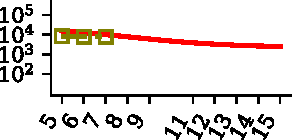
\includegraphics[width=\linewidth]{figure/soc-pokec-relationships_r4_memory_by_s_no_hi.pdf}
    \caption{PO $s\{r{=}4\}$}
  \end{subfigure}
  \caption{Time and Memory usage comparison for ($r \in \{1,2,3,4\}$).}
  \label{fig:mem_panel_b}
\end{figure*}
}


\section{Experimental Evaluation} \label{sec:exp}

\stitle{Hardware.} All algorithms are implemented in C++ and compiled using the g++ compiler with -O3 optimization. 
Experiments were conducted on a machine equipped with dual Intel(R) Xeon(R) Gold 6342 2.80GHz CPUs, 500GB of RAM, and running Ubuntu 22.

\input{sections/datasetTable}

% \renewcommand{\tabcolsep}{6pt}
\stitle{Datasets.} We evaluate our approach on six real-world datasets from diverse domains, including Co-authorship Networks: \textit{com-dblp} (cblp)~\cite{dblp}; Social Networks: \textit{soc-pokec} (pokec)~\cite{soc-pokec}, \textit{com-youtube} (youtube)~\cite{dblp}; and Web Graphs: \textit{web-Google} (google)~\cite{Stanford}, \textit{web-it-2004} (web-it)~\cite{nr}, \textit{web-Stanford} (stanford)~\cite{Stanford}. These datasets vary in size and structural characteristics, providing a comprehensive evaluation of our approach. Table~\ref{tab:graph-stats} summarizes the key statistics of these datasets.
% , including the number of vertices ($n$), number of edges ($m$), average degree, maximum degree, and the number of triangles. The datasets range from hundreds of thousands to over a million vertices, with varying edge densities and triangle counts, reflecting their diverse nature.

\stitle{Algorithms.} 
\myaddRA{
We compare our method with two state-of-the-art methods from the ARB line: the peeling framework \arb without hierarchy \cite{sotaPrveHierarchy}\footnote{\url{https://github.com/jeshi96/arb-nucleus-decomp}} and its hierarchy construction extension \cite{sotaHierarchy}\footnote{\url{https://github.com/jeshi96/arb-nucleus-hierarchy}}.
}
and the local $h$-index framework \nucleus from~\cite{LocalNuclear}\footnote{\url{https://github.com/sariyuce/nucleus}}.
\myaddRA{For \nucleus, in addition to its base implementation, we also evaluate its two optimized parallel variants available in the same repository: the peeling-based \nucleusP and the optimized local $h$-index \nucleusOPT.}
\arb, \nucleus and our method support hierarchy construction and core decomposition, while the \nucleusOPT and \nucleusP focus on decomposition.
% 
Notably, \arb does not support $r=1$ due to its algorithmic design. 
% 
Regarding \nucleus, its base implementation only supports the cases of $(r,s)=(1,3)$, $(1,4)$, $(2,3)$, and $(3,4)$.
% 这里紧接着说明优化版限制更死：只支持 (3,4)
\myaddRA{
Furthermore, \nucleusP and \nucleusOPT, are even more specialized and only support the case of $(r,s)=(3,4)$.
}
% 
Our method is publicly available.\footnote{\url{https://github.com/JamesZwq/nuclearSigmod/}}
%
Although these baselines differ in implementation details, they all follow the same exact peeling skeleton reviewed in Section~\ref{sec:existing_approaches} and rely on more reconstructive support-maintenance primitives.
%
They differ in implementation.
%
But they use the same exact peeling skeleton reviewed in Section~\ref{sec:existing_approaches}.
%
They also use more reconstructive support-maintenance primitives.
%
Our end-to-end comparison therefore evaluates both layers of our method.
%
It evaluates the counting/index layer provided by \cpi.
%
It also evaluates the DPCM update layer introduced in Section~\ref{sec:dpcm}.


\stitle{Metrics.}
Each experiment is executed three times, and we report the \emph{average} wall-clock runtime. 
A timeout of \textbf{3600\,seconds} (1 hour) is imposed; runs exceeding this limit are marked as \emph{out of time (OOT)} (denoted by $\textcolor{red}{\boldsymbol{\times}}$ in figures) and excluded from the averages.

\stitle{Evaluation Questions.}
Our experiments are designed to answer four questions.
%
\textbf{Q1:} Does the combined \cpi\,+\,DPCM framework consistently outperform prior exact peeling methods across different values of $r$ and $s$?
%
\textbf{Q2:} Do the three DPCM instantiations yield the expected regime-specific benefits, namely counter-state updates for $r{=}1$, edge-contribution updates for $r{=}2$, and conflict-state pruning for $r{\ge}3$?
%
\textbf{Q3:} How much of the gain comes from avoiding reconstructive support maintenance, as opposed to merely changing the underlying representation?
%
\textbf{Q4:} Does the same framework also preserve the efficiency advantage when hierarchy construction is included?
%
Questions~Q1--Q3 separate the two layers of our approach.
%
Q1 studies the end-to-end effect of combining representation and maintenance.
%
Q2 studies whether the regime-specific sufficient states predicted by DPCM appear in practice.
%
Q3 separates the compression benefit of \cpi from the update benefit of differential maintenance.
%
Q4 checks whether the same advantages remain after we add connectivity maintenance for hierarchy construction.

% In line plots, \emph{out-of-time (OOT)} cases are indicated by a red patterned band at the timeout threshold; accordingly, any red pattern along the top of the plot denotes an OOT case. And for all following experiments, we run the experiment until the first timeout for all methods(e.g., if one method times out at $s=4$, we will not run the experiment for $s>4$ for this method).


% \expsection{Running Time $(r \leq 2)$}
% % 在本试验中, 我们运行了table~\ref{tab:graph-stats}中列出的六个真实数据集, 并分别测试了在没有hierarchical构建的$r=1$和$r=2$的情况. 对于每个数据集, 我们将参数$s$从较小的值(例如$r=1$时的$s=3$, $r=2$时的$s=4$)逐步增加到数据集中观察到的最大团大小. 实验结果如图~\ref{fig:dblp_r1_time_by_s}所示. 我们的算法CND在任何数据集中, 随着$s$的增加, 运行时间并无显著增长, 并且曲线趋于平稳, 我们高效的计算了所有s的结果. 
% In this experiment, we evaluate both $r=1$ and $r=2$ cases without hierarchical construction across six datasets. 
% For each dataset, we vary the parameter $s$ from small values (e.g., $s=3$ for $r=1$ and $s=4$ for $r=2$) up to the maximum clique size in the dataset. 
% The experimental results are shown in Figure~\ref{fig:r1r2_time_by_s}. 
% Across all datasets, as $s$ increases, the runtime of our \cbnd algorithm exhibits minimal growth and quickly stabilizes, demonstrating its ability to efficiently compute results for all values of $s$.
% % 算法\arb和算法\nucleus在大多数情况下, 运行时间都随着s的增加有着显著增长并且快速timeout. 算法\arb在youtube 数据集r=2的时候有着不寻常的表现, 因为youtube 数据集的最大团大小为17, 很小, 所以我们的算法在这个数据集上的优势并不太明显, 但是其在r=2,s=13时也timeout, 对比之下, CND只是用了30秒就完成了计算.
% \arb and \nucleus exhibit substantial runtime growth as $s$ increases in most cases, often leading to rapid timeouts. 
% Notably, \arb performs better on the \textsc{YouTube} dataset for $r=2$, as its maximum clique size is small (i.e., $17$). 
% Consequently, the performance gap between \arb and our algorithm is narrower on this dataset. 
% However, \arb still times out at $r=2, s=13$, whereas \cbnd completes the computation in only 30 seconds.
% % 
% % 在数据集web-it-2004上, ARB在r=2的任何s下都timeout了, 而CND在r=2,s=4的情况下只用了240秒就完成了计算, 并且顺利的计算了所有s的结果.
% On the \textsc{web-it-2004} dataset, \arb times out for all values of $s$ when $r=2$, whereas \cbnd completes the computation in only 240 seconds for $r=2, s=4$, successfully producing results for all values of $s$.
% % 在本试验中 CND比ARB和NUCLEUS分别有平均30x和20x的加速, 对快达到了342x在dblp数据集的r=2,s=5的情况下.
% \cbnd achieves average speedups of 30x and 20x over \arb and \nucleus, respectively, with a maximum speedup of 342x observed on the DBLPdataset for $r=2, s=5$.

\expsection{Running Time $(r \leq 2)$}
We evaluate $r\in\{1,2\}$ without hierarchy on six datasets, sweeping $s$ from $3/4$ up to each dataset's maximum clique size (Figure~\ref{fig:r1r2_time_by_s}).
%
These results answer Q1.
%
They also answer the low-order part of Q2.
%
\cbnd shows little sensitivity to $s$: curves are essentially flat across datasets.
%
This is the behavior predicted by counter-state and edge-contribution DPCM.
%
Once \cpi compactly represents the clique space, support updates do not need to reconstruct large affected local neighborhoods as $s$ grows.
%
In contrast, \arb and \nucleus grow rapidly with $s$ and often time out.
%
Atypical is \texttt{com-youtube} at $r{=}2$ (max clique $17$), where the gap narrows; even there, \arb times out at $s{=}13$ while \cbnd finishes in about 30s.
%
On \texttt{web-it-2004} ($r{=}2$), \arb times out for all $s$, whereas \cbnd completes from $s{=}4$ onward (e.g., 240s at $s{=}4$) and handles the full range.
%
On comparable settings, \cbnd is about $6.3\times$ faster than \arb and about $18.0\times$ faster than \nucleus.
%
The largest gap is above two orders of magnitude.
% 
% 我们也与目前最先进的kcore和ktruss的算法进行了对比, 
\myaddRA{
We further compare against specialized single-thread baselines for the two canonical special cases: $k$-core ($(r,s)=(1,2)$)\cite{batagelj2003omalgorithmcoresdecomposition} and $k$-truss ($(r,s)=(2,3)$)\cite{wang2012truss}. 
On \texttt{com-dblp}, \cbnd runs in $1.21$s for $(1,2)$ vs.\ $0.45$s for $k$-core, and $1.31$s for $(2,3)$ vs.\ $0.78$s for $k$-truss. 
This result shows that our combined CPI+DPCM framework has only modest overhead on the special cases.
%
It still keeps the advantage of avoiding explicit clique enumeration.
%
It also remains effective as $s$ increases.
}


\expsection{Running Time $(r \in \{3,4\})$}
We evaluate $r\in\{3,4\}$ on three datasets, with and without hierarchy (Figure~\ref{fig:time_by_s_r3_r4_combined}).

\expsubsection{Without Hierarchy}
Figure~\ref{fig:time_by_s_r3_r4_combined} compares \cbnd with \nucleus and \arb. 
%
This part mainly answers the general-regime side of Q2.
%
It also helps answer Q3.
%
As with $r\le 2$, \cbnd is nearly insensitive to $s$, curves stay essentially flat, while \arb (and \nucleus) grow rapidly with $s$ and frequently time out. 
%
The key difference is that the gain here does not come from simple counter or edge states.
%
It comes from conflict-state DPCM.
%
Dead paths are pruned early.
%
Only the surviving residual paths need further exact maintenance.
%
On comparable settings, \cbnd is about $2.8\times$ faster than \arb and about $4.6\times$ faster than the base \nucleus implementation.
%
The largest speedup reaches $106.7\times$ on \texttt{com-dblp} at $r{=}3, s{=}5$.
% 新增对比
\myaddRA{
We also evaluate the specialized algorithms \nucleusP and \nucleusOPT for $(r,s)=(3,4)$. 
On \texttt{com-dblp}, \cbnd achieves $3.2\times$ and $5.5\times$ speedups, respectively.
% 简短的原因分析
However, \cbnd is less effective on graphs with small max cliques but large average degrees (e.g., \texttt{soc-pokec} and \texttt{web-Google}).
% 在这两个数据集中, (r,s)=(3,4)的时候,\nucleusOPT, \nucleusP和\arb均比CND快了1点多倍, 当然随着s的增加, 例如(3,5)和(4,5)的时候,CND有迅速获得了强大的优势.
In these datasets, for $(r,s)=(3,4)$, \nucleusOPT, \nucleusP, and \arb are all around $1\times$ faster than \cbnd; however, as $s$ increases (e.g., $(3,5)$ and $(4,5)$), \cbnd quickly gains a strong advantage.
% 这是因为在
In such cases, the enumeration cost for baselines is naturally low, while the dense connectivity increases the maintenance overhead of our index.
}

\expsubsection{With Hierarchy}
Figure~\ref{fig:time_by_s_r3_r4_combined}.2 shows the hierarchical setting.
%
This addresses Q4.
%
The same trend appears in the hierarchical setting.
%
\cbnd stays stable as $s$ increases, whereas the baselines often slow down or time out.
%
On comparable settings, \cbnd is about $2.6\times$ faster than \arb and about $18.4\times$ faster than \nucleus.
%
The largest speedup reaches $146.6\times$ on \texttt{com-dblp} at $r{=}3, s{=}4$.

\expsection{Running Time $(r \in \{5,6,7\})$}
\myaddRA{
Figure~\ref{fig:time_by_s_r5_r7_combined} reports the efficiency for higher-order nucleus decomposition on \texttt{soc-pokec} and \texttt{com-youtube}. 
As $r$ increases, \cbnd maintains a robust and relatively flat performance curve. 
In contrast, \arb exhibits a non-monotonic trend. 
On \texttt{soc-pokec}, the speedup of \cbnd over \arb narrows at medium $r$ (e.g., dropping to $1.0\times$ at $r{=}6$), as stricter constraints shrink the search space for enumeration.
However, this resilience is transient. 
At $r{=}7$, \arb degrades sharply on \texttt{soc-pokec} (e.g., taking 2590s at $s{=}11$ vs. 31s for \cbnd, an $83\times$ difference) and eventually times out. 
The situation is even worse on \texttt{com-youtube}, where \arb fails to complete entirely at $r{\ge}7$.
This demonstrates that while enumeration-based frameworks can transiently benefit from filtered search spaces, they remain fundamentally fragile to high-order complexity.
}


\begin{figure}
  \centering
  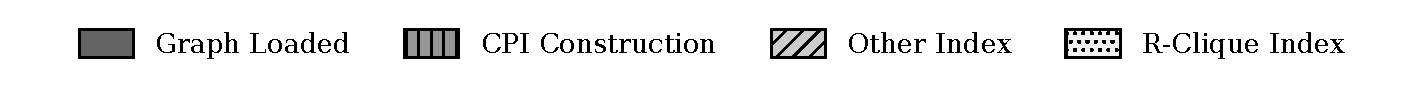
\includegraphics[width=0.7\textwidth]{figure/breakdown_memory_legend.pdf}
  

  \begin{subfigure}[t]{0.32\textwidth}
      \centering
      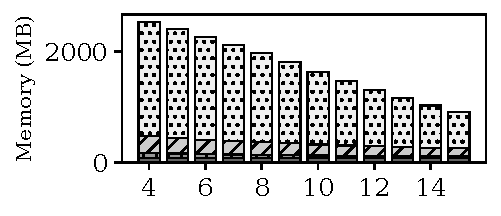
\includegraphics[width=\linewidth]{figure/breakdown_memory_Google.pdf}
      \caption{GO $s\{r{=}3\}$}
      \label{fig:bd_google_mem}
  \end{subfigure}\hfill
  \begin{subfigure}[t]{0.32\textwidth}
      \centering
      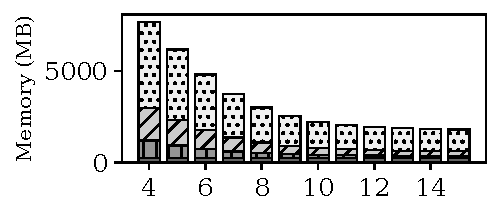
\includegraphics[width=\linewidth]{figure/breakdown_memory_Pokec.pdf}
      \caption{PO $s\{r{=}3\}$}
      \label{fig:bd_pokec_mem}
  \end{subfigure}\hfill
  \begin{subfigure}[t]{0.32\textwidth}
      \centering
      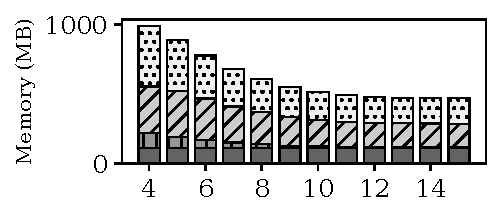
\includegraphics[width=\linewidth]{figure/breakdown_memory_Youtube.pdf}
      \caption{YT $s\{r{=}3\}$}
      \label{fig:bd_youtube_mem}
  \end{subfigure}
    \caption{Breakdown of \textbf{memory usage} on different datasets ($r=3$) as $s$ varies. }
  \label{fig:breakdown_mem}
  
  \centering
  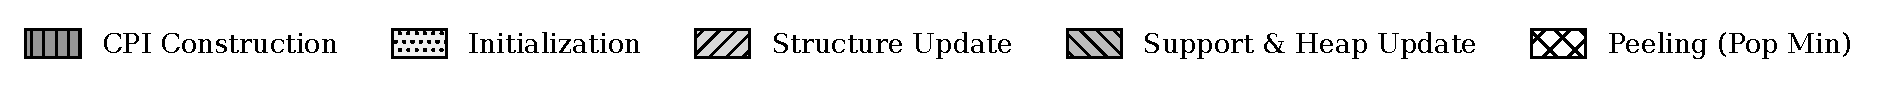
\includegraphics[width=0.9\textwidth]{figure/breakdown_legend.pdf}

  \begin{subfigure}[t]{0.32\textwidth}
      \centering
      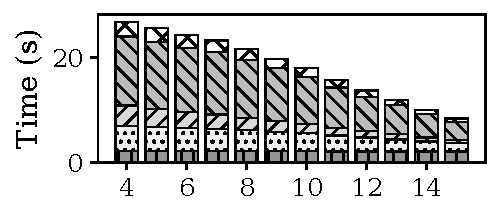
\includegraphics[width=\linewidth]{figure/breakdown_Google.pdf}
      \caption{GO $s\{r{=}3\}$}
      \label{fig:bd_google_time}
  \end{subfigure}\hfill
  \begin{subfigure}[t]{0.32\textwidth}
      \centering
      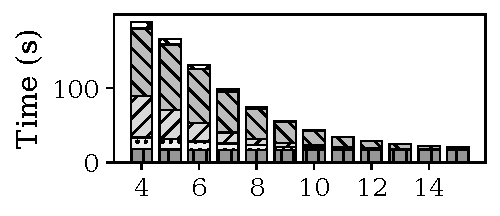
\includegraphics[width=\linewidth]{figure/breakdown_Pokec.pdf}
      \caption{PO $s\{r{=}3\}$}
      \label{fig:bd_pokec_time}
  \end{subfigure}\hfill
  \begin{subfigure}[t]{0.32\textwidth}
      \centering
      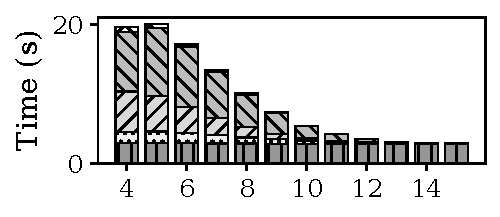
\includegraphics[width=\linewidth]{figure/breakdown_Youtube.pdf}
      \caption{YT $s\{r{=}3\}$}
      \label{fig:bd_youtube_time}
  \end{subfigure}
    \caption{Breakdown of \textbf{running time} on different datasets ($r=3$) as $s$ varies. }
  \label{fig:breakdown_time}
\end{figure}


\expsection{Memory Usage}
\myaddRA{
Figures~\ref{fig:mem_panel_b}(a-i) and~\ref{fig:breakdown_mem} analyze memory consumption. Our method and the state-of-the-art \arb have comparable memory usage overall. As $s$ increases, our memory decreases while \arb stays nearly constant.
This is because larger $s$ leaves fewer valid $r$-cliques: many $r$-cliques contain no $s$-cliques. We do not store such $r$-cliques, whereas \arb cannot reliably pre-filter them and thus maintains states for all $r$-cliques.
% 
For $r{=}1$, our method uses more memory than \nucleus but is substantially faster. 
On \texttt{com-dblp} ($r{=}1,s{=}4$), \nucleus uses 73MB and takes 62.8s, while our method uses 253MB ($\approx3.5\times$) and finishes in 0.8s (77.7$\times$ speedup). 
On \texttt{web-Stanford} ($r{=}1,s{=}3$), \nucleus uses 126MB and runs for 596s, while our method uses 656MB and completes in 55s (x10.8$\times$ speedups). 
Thus, even in low-order settings where baselines are optimized, the additional memory translates to significant performance gains.
}
\myaddRC{
Figure~\ref{fig:breakdown_mem} further breaks down \cbnd's memory usage across datasets and $(r,s)$ settings. Most memory is spent on storing $r$-cliques rather than CPI, indicating that \cpi itself is memory-efficient.
}




\expsection{Runtime Breakdown}
\myaddRA{
Figure~\ref{fig:breakdown_time} reports the runtime breakdown of \cbnd across datasets. 
We decompose the total time into five components:
\textit{CPI Construction},
\textit{Init} (initial $r$-clique enumeration and support counting),
\textit{Structure Update} (updating CPI structure during peeling),
\textit{Support} (updating $s$-clique supports via neighbor intersections),
and \textit{Peeling} (heap maintenance and PopMin operations).
Overall, \textit{Init} and \textit{Support} are the main cost drivers.
On \texttt{com-dblp} ($r{=}4$), \textit{Init} accounts for 36.2\%--38.0\% and \textit{Support} for 17.7\%--18.3\% (two runs); on \texttt{web-Google} ($r{=}4$), \textit{Support} becomes the bottleneck (39.9\%) while \textit{Init} is 14.5\% (and \textit{Peeling} is 27.3\%).
These results indicate that runtime is primarily governed by clique enumeration and neighbor intersections (Init/Support), while CPI construction/maintenance and heap-based peeling contribute the remaining overhead.
%
For Q3, the important observation is that \textit{Structure Update} remains a secondary cost across datasets.
%
This is consistent with DPCM: once the initial representation is built, most dynamic work is handled by localized differential updates rather than repeated reconstructive maintenance of the full affected clique space.
}


\begin{figure}

  
  \centering
  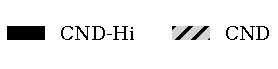
\includegraphics[width=0.2\linewidth]{figure/cbs_vs_nohi_comp_legend_long.pdf}
  

  \begin{subfigure}[t]{0.243\textwidth}
    \centering 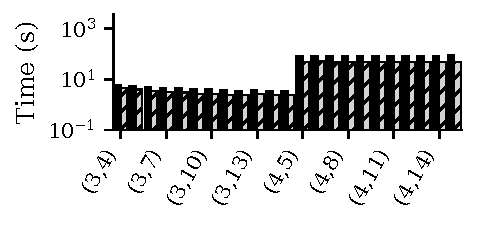
\includegraphics[width=\linewidth]{figure/abc_comp_com-dblp_time_by_rs_long.pdf}
    \caption{DBLP($r$,$s$)}
  \end{subfigure}
  \begin{subfigure}[t]{0.243\textwidth}
    \centering 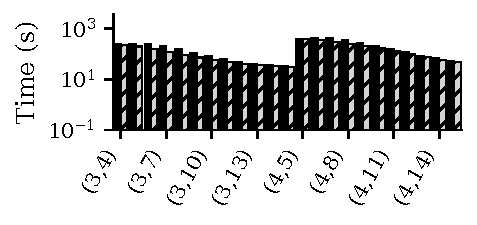
\includegraphics[width=\linewidth]{figure/abc_comp_soc-pokec-relationships_time_by_rs_long.pdf}
    \caption{PO ($r$,$s$)}
  \end{subfigure}
  \begin{subfigure}[t]{0.243\textwidth}
    \centering 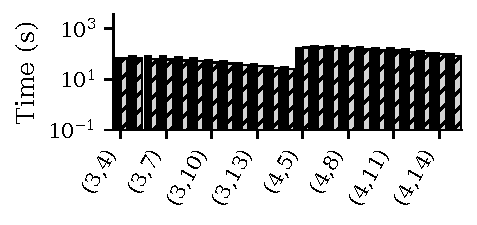
\includegraphics[width=\linewidth]{figure/abc_comp_web-Google_time_by_rs_long.pdf}
    \caption{GO ($r$,$s$)}
  \end{subfigure}
  \begin{subfigure}[t]{0.243\textwidth}
    \centering 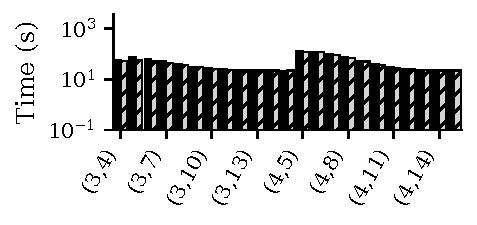
\includegraphics[width=\linewidth]{figure/abc_comp_com-youtube_time_by_rs_long.pdf}
    \caption{YT ($r$,$s$)}
  \end{subfigure}

  \caption{Time (in seconds) Hierarchical vs Non-Hierarchical with varying $r,s$.}
  \label{fig:hierarchy_vs_nohierarchy}
\end{figure}

\begin{figure}
  \centering
  
\includegraphics[width=0.50\linewidth]{figure/legend_leafCount_generic.pdf}
    
  \begingroup
  \setcounter{panel}{0}
  \begin{minipage}[c]{0.02\textwidth}
    \centering
      \raisebox{4em}{\rotatebox{90}{\tiny \textbf{Count}}} 
  \end{minipage}    \begin{subfigure}[t]{0.16\textwidth} 
      \centering 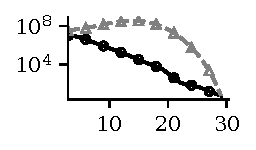
\includegraphics[width=\linewidth]{figure/leaf_clique_soc-pokec-relationships.pdf}
      % \caption{$k$-clique \\ (pokec)}
      \caption{PO $k$-clique}
    \end{subfigure}\hfill
    \begin{subfigure}[t]{0.16\textwidth}
      \centering 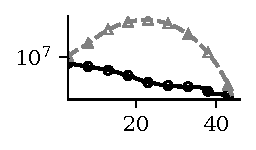
\includegraphics[width=\linewidth]{figure/leaf_clique_web-Google.pdf}
      % \caption{$k$-clique \\ (Google)}
      \caption{GO $k$-clique}
    \end{subfigure}\hfill
    \begin{subfigure}[t]{0.16\textwidth}
      \centering 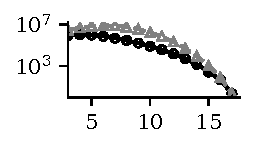
\includegraphics[width=\linewidth]{figure/leaf_clique_com-youtube.pdf}
      % \caption{$k$-clique \\ (youtube)}
      \caption{YT $k$-clique}
    \end{subfigure}\hfill
    \begin{subfigure}[t]{0.16\textwidth}
      \centering 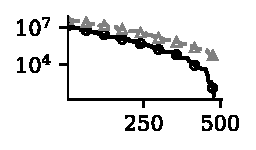
\includegraphics[width=\linewidth]{figure/leafCount_soc-pokec-relationships_34.pdf}
      % \caption{\#Iter \\ (pokec)}
      \caption{PO \#Iter}
    \end{subfigure}\hfill
    \begin{subfigure}[t]{0.16\textwidth}
      \centering 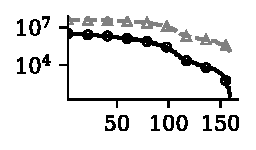
\includegraphics[width=\linewidth]{figure/leafCount_web-Google_34.pdf}
      % \caption{\#Iter \\ (Google)}
      % \caption{\#Iter \\ (GO)}
      \caption{GO \#Iter}
    \end{subfigure}\hfill
    \begin{subfigure}[t]{0.16\textwidth}
      \centering 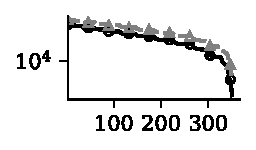
\includegraphics[width=\linewidth]{figure/leafCount_com-youtube_34.pdf}
      % \caption{\#Iter \\ (youtube)}
      \caption{YT \#Iter}
    \end{subfigure}\hfill

  
  \caption{CPI \#Paths vs.\ \#s-cliques for $r=3, s=4$.}
    \label{fig:leafcount}
    
  \endgroup
\end{figure}





\expsection{Ablation Study for $r \in {1,2}$}
\myaddRA{
Figure~\ref{fig:ablation_exp} reports an ablation study for $r\in\{1,2\}$.
To reduce the overhead of generic clique enumeration at low orders, we add specialized optimizations for $r{=}1$ and $r{=}2$.
Compared with the generic baseline (\texttt{CBS3}), the optimized version (\texttt{CBS-noHi}) is consistently faster:
on \texttt{com-dblp} with $r{=}2,s{=}4$, runtime drops from 1.57s to 1.04s (1.5$\times$), and for $r{=}1$ we observe $\approx$1.3$\times$ speedup.
Memory usage remains similar since the optimization only changes \cpi updates and does not change the stored \cpi structure.
%
This directly supports Q2: once the same \cpi representation is fixed, regime-specific DPCM operators still contribute additional gains.
}




\begin{figure}
  \centering
      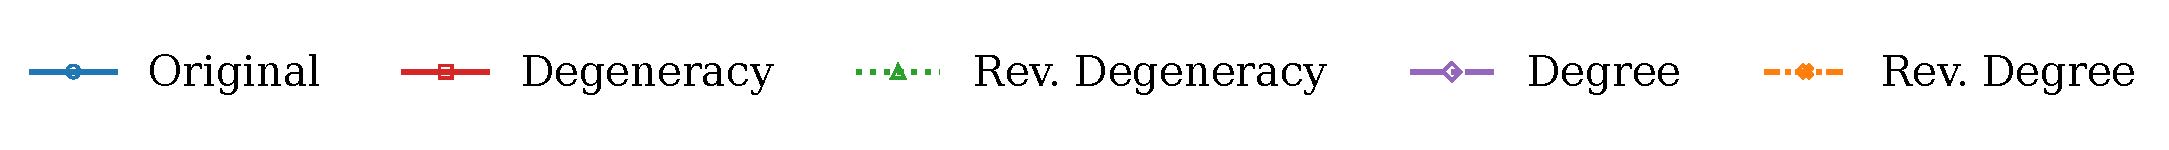
\includegraphics[width=0.8\linewidth,trim={0 8pt 0 26pt},clip]{figure/legend_sort_options.pdf}
  
      \setlength{\tabcolsep}{0pt} 
    \begin{subfigure}[t]{0.162\textwidth}
    \centering
    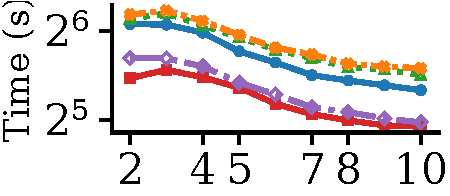
\includegraphics[width=\linewidth]{figure/r1_time.pdf}
    \caption{$s\{r{=}1\}$ \\ Time}
    \label{fig:ord_r1_time}
  \end{subfigure}\hfill
  \begin{subfigure}[t]{0.162\textwidth}
    \centering
    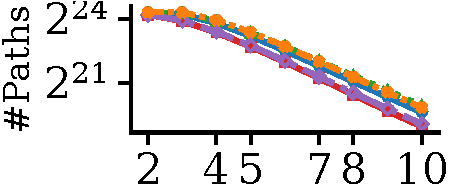
\includegraphics[width=\linewidth]{figure/r1_leafs.pdf}
    \caption{$s\{r{=}1\}$ \\ \#Paths}
    \label{fig:ord_r1_mem}
  \end{subfigure}\hfill
  \begin{subfigure}[t]{0.162\textwidth}
    \centering
    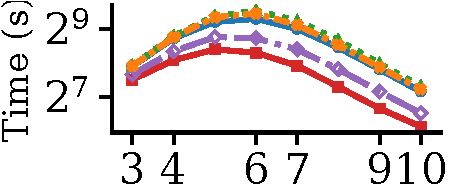
\includegraphics[width=\linewidth]{figure/r2_time.pdf}
    \caption{$s\{r{=}2\}$ \\ Time}
    \label{fig:ord_r2_time}
  \end{subfigure}\hfill
  \begin{subfigure}[t]{0.162\textwidth}
    \centering
    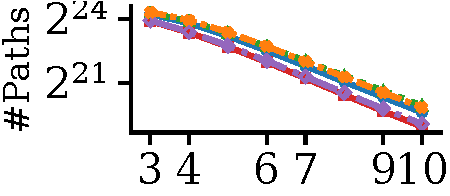
\includegraphics[width=\linewidth]{figure/r2_leafs.pdf}
    \caption{$s\{r{=}2\}$ \\ \#Paths}
    \label{fig:ord_r2_mem}
  \end{subfigure}\hfill
    \begin{subfigure}[t]{0.162\textwidth}
    \centering
    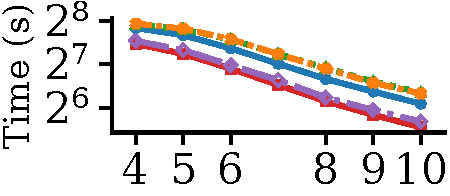
\includegraphics[width=\linewidth]{figure/r3_time.pdf}
    \caption{$s\{r{=}3\}$ \\ Time}
    \label{fig:ord_r3_time}
  \end{subfigure}\hfill
  \begin{subfigure}[t]{0.162\textwidth}
    \centering
    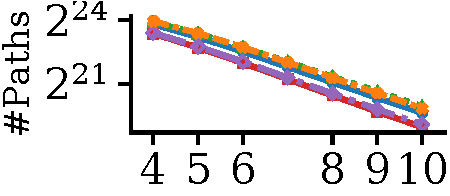
\includegraphics[width=\linewidth]{figure/r3_leafs.pdf}
    \caption{$s\{r{=}3\}$ \\ \#Paths}
    \label{fig:ord_r3_mem}
  \end{subfigure}\hfill

    \caption{Impact of different vertex ordering strategies in soc-pokec}
  \label{fig:order_exp}
  
\end{figure}


\expsection{Hierarchy vs.\ No Hierarchy}
% 在本试验中我们对比了我们的算法CND在有和没有hierarchical构建的情况下的性能差异.
% In this experiment, we compare the performance of our \cbnd algorithm with and without hierarchical construction.
% 图~\ref{fig:hierarchy_vs_nohierarchy}展示了在$r=3$和$r=4$的情况下, 我们的算法CND在有和没有hierarchical构建的情况下的对比. 我们选择了数据集dblp, soc-pokec-relationships和web-Google作为代表.
% Figure~\ref{fig:hierarchy_vs_nohierarchy} illustrates the comparison of our \cbnd algorithm with and without hierarchical construction for $r=3$ and $r=4$. We select the datasets \texttt{Youtube}, \texttt{soc-pokec}, and \texttt{web-Google} as representatives.
% Across all datasets, the runtimes of our \cbnd algorithm with and without hierarchical construction are very close. On average, the hierarchical version takes about 10\% more time than the non-hierarchical version. This indicates that our \cbnd algorithm exhibits very stable performance regardless of whether hierarchical construction is employed.
Figure~\ref{fig:hierarchy_vs_nohierarchy} compares \cbnd with and without hierarchical construction for $r\in\{3,4\}$ on \texttt{Youtube}, \texttt{soc-pokec}, and \texttt{web-Google}.
Across all three datasets, the two variants have nearly identical runtimes; the hierarchical version is about 10\% slower on average.
This indicates that our \cbnd algorithm exhibits very stable performance regardless of whether hierarchical construction is employed.
%
This confirms Q4: once \cpi and DPCM are in place, maintaining $s$-connectivity for hierarchy adds only modest overhead.




\begin{figure}
  \centering

    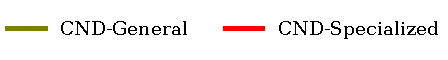
\includegraphics[width=0.4\linewidth]{figure/special_cbs_comparison_legend-eps-converted-to.pdf}
  
  \captionsetup[subfigure]{font=tiny, skip=0pt}
  
  \begin{subfigure}[t]{0.24\textwidth}
    \centering
    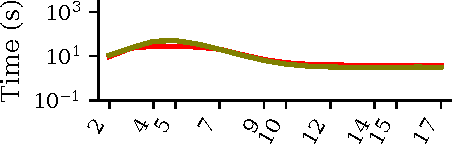
\includegraphics[width=\linewidth]{figure/special_com-youtube_r1_time.pdf}
    \caption{YT $s\{r{=}1\}$}
  \end{subfigure}\hfill
  \begin{subfigure}[t]{0.24\textwidth}
    \centering
    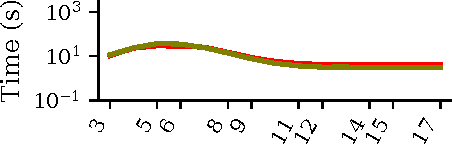
\includegraphics[width=\linewidth]{figure/special_com-youtube_r2_time.pdf}
    \caption{YT $s\{r{=}2\}$}
  \end{subfigure}\hfill
  \begin{subfigure}[t]{0.24\textwidth}
    \centering
    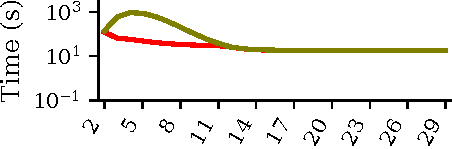
\includegraphics[width=\linewidth]{figure/special_soc-pokec-relationships_r1_time.pdf}
    \caption{PO $s\{r{=}1\}$}
  \end{subfigure}\hfill
  \begin{subfigure}[t]{0.24\textwidth}
    \centering
    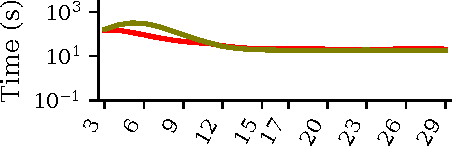
\includegraphics[width=\linewidth]{figure/special_soc-pokec-relationships_r2_time.pdf}
    \caption{PO $s\{r{=}2\}$}
  \end{subfigure}\hfill
  \begin{subfigure}[t]{0.24\textwidth}
    \centering
    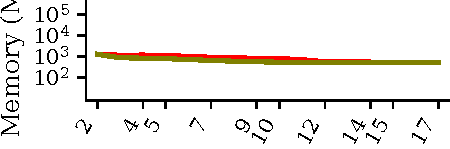
\includegraphics[width=\linewidth]{figure/special_com-youtube_r1_mem.pdf}
    \caption{YT $s\{r{=}1\}$}
  \end{subfigure}\hfill
  \begin{subfigure}[t]{0.24\textwidth}
    \centering
    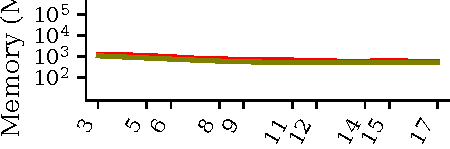
\includegraphics[width=\linewidth]{figure/special_com-youtube_r2_mem.pdf}
    \caption{YT $s\{r{=}2\}$}
  \end{subfigure}\hfill
  \begin{subfigure}[t]{0.24\textwidth}
    \centering
    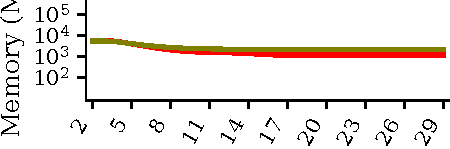
\includegraphics[width=\linewidth]{figure/special_soc-pokec-relationships_r1_mem.pdf}
    \caption{PO $s\{r{=}1\}$}
  \end{subfigure}\hfill
  \begin{subfigure}[t]{0.24\textwidth}
    \centering
    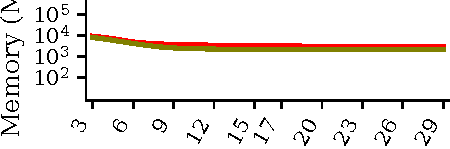
\includegraphics[width=\linewidth]{figure/special_soc-pokec-relationships_r2_mem.pdf}
    \caption{PO $s\{r{=}2\}$}
  \end{subfigure}\hfill
                                                                                  

    \caption{Comparison of execution time for \cbnd general vs. specialized algorithms.}
  \label{fig:ablation_exp}
  
\end{figure}

\expsection{Node Orderings}
\myaddRB{
We evaluate five vertex orderings on \texttt{soc-pokec} (Figure~\ref{fig:order_exp}): \texttt{origin}, \texttt{degree}/\texttt{degreeR}, and \texttt{degen}/\texttt{degenR}.
Across all tested $s$ (2--10 for $r{=}1$, 3--10 for $r{=}2$, and 4--10 for $r{=}3$), \texttt{degen} is consistently the best overall.
Averaged over all tested $s$, \texttt{degen} is
1.39$\times$ faster than \texttt{origin} for $r{=}1$ (52.6s $\rightarrow$ 37.9s),
1.86$\times$ for $r{=}2$ (392.5s $\rightarrow$ 210.5s), and
1.37$\times$ for $r{=}3$ (139.8s $\rightarrow$ 102.1s).
% The second-best choice is typically \texttt{degree}, but \texttt{degen} still yields an extra 7.3\% / 23.3\% / 6.0\% speedup for $r{=}1/2/3$.
In contrast, the reverse orderings are consistently the slowest: \texttt{degenR}/\texttt{degreeR} are 1.52--2.11$\times$ slower than \texttt{degen} on average.
% 
Moreover, \texttt{degen} shrinks the CPI: compared with \texttt{origin}, it reduces CPI \#paths by 28.3\% / 30.9\% / 32.5\% on average for $r{=}1/2/3$ (up to 37.2\% at $s{=}10$), translating to average memory savings of 0.82 / 0.67 / 0.37\,GB.
For example, at $r{=}1,s{=}3$, \texttt{degen} reduces CPI \#paths from 19.78M to 15.82M ($-20\%$), lowering memory from 6.35\,GB to 5.18\,GB ($-1.17$\,GB) and runtime from 67.2s to 47.3s.
We therefore adopt \texttt{degen} as the default ordering strategy.
}


\expsection{\#Paths vs. \#$s$-Cliques}
Across peeling iterations, we compare the number of CPI paths with the number of $s$-cliques (Figure~\ref{fig:leafcount}) for $(r,s)=(3,4)$ on three datasets. 
On all datasets and in almost all iterations, the path count is far below $|K_s|$, indicating that CPI stays compact and output-sensitive.
Moreover, the path count is flat or decreasing over time, suggesting that path splits are non-inflationary.
A mild exception is \texttt{com-youtube} at $s{=}4$, whose sparsity and small maximum clique size ($\omega{=}17$) narrow the gap, consistent with its more modest speedups (Figure~\ref{fig:youtube_r2_time_by_s}).
%
This experiment isolates the representation side of Q3: even before considering differential updates, \cpi already compresses the active clique space substantially.


% 
% \expsection{Scalability}
% We evaluate scalability on \texttt{web-Google} and \texttt{youtube}(Figure~\ref{fig:scalability_time_memory}).
% For each graph, we run $r\in\{1,2,3\}$ and sweep $s$ up to 15, reporting wall-clock time. 
% We vary workload by subsampling edges to 20--100\% of the input; the curves are labeled by sampling ratios. 
% Runtime curves are cleanly ordered (20\% $<$ 40\% $<$ 60\%$< $80\%$<$100\%), indicating near-linear dependence on graph size. 
% Moreover, time consistently decreases as $s$ increases, and this trend holds even at 100\% input, demonstrating robust full-scale performance. 
% Overall, \cbnd scales smoothly with both graph size and parameters.

\myaddRA{
\expsection{Stress Test}
% To evaluate limits under combinatorial explosion, To probe the limits under combinatorial explosion, we stress-test synthetic graphs ($N{=}1000$) generated via incremental clique injection, where clique sizes follow a truncated power-law and the injected clique size is capped at 100; we vary the edge density from $p{=}0.01$, yielding $deg_{\text{avg}}\approx p|V|$.
 To evaluate limits under combinatorial explosion, We stress-test on $N{=}1000$ synthetic graphs built by incremental clique injection: clique sizes are sampled from a truncated power-law (max size $100$), and density is increased from $p{=}0.01$, yielding $\bar d \approx p(|V|-1)$.
It is worth noting that our starting density $p{=}0.01$ is already orders of magnitude higher than typical real-world networks (e.g., \texttt{com-dblp} has $p{\approx}2{\times}10^{-5}$), creating a rigorous worst-case scenario.
Experimental results ($r{\in}\{4,5\}, s{\in}\{5..9\}$) show that \cbnd remains robust in these settings.
As complexity increases, the baseline \arb collapses rapidly: for $(r,s){=}(4,7)$, it times out at a mere $p{=}0.05$, and for $s{\ge}8$, it fails immediately at $p{=}0.01$.
In contrast, \cbnd robustly processes densities up to $p{=}0.20$ across all settings.
For $(r,s){=}(4,6)$ at $p{=}0.11$, \cbnd achieves a 210$\times$ speedup (30s vs. 6310s).
Regarding memory, although \cbnd consumes higher memory than \arb ($\approx 2.3\times$), the usage ratio remains constant as density increases.
This linear scaling indicates that our index structure effectively withstands the exponential growth of redundant cliques that paralyzes enumeration-based methods.

\sstitle{Leaf cliques vs.\ total cliques.}
% For each density $p$, the number of path and the total number of $k$-cliques, as a function of clique size $k$.
As $p$ increases, the peak path in \cpi count grows and shifts to larger $k$ (e.g., from $999$ at $k{=}3$ when $p{=}0.01$, to $2.98\times 10^{9}$ at $k{=}10$ when $p{=}0.38$),
but the total $k$-clique count grows much faster and becomes infeasible to enumerate.
For example, at $p{=}0.01$ there are $3.53\times 10^{10}$ 20-cliques but only $46$ leaf cliques of size 20; at $p{=}0.38$ there are $8.41\times 10^{27}$ 49-cliques but only $4{,}028$ leaf cliques of size 49.
This shows that even under extremely dense graphs, CPI still achieves a high compression ratio.



\sstitle{Suggestion for algorithm selection.}
Our recommendation is simple: \arb is competitive for \emph{low-order} settings on \emph{very dense} graphs (e.g., $r{=}4,s{=}5,p{>}0.18$) and uses less memory.
In most other regimes---\emph{sparser} graphs ($p{<}0.18$) or \emph{higher-order} settings ($r{\ge}5,s{\ge}6$)---we recommend \cbnd, which consistently achieves large speedups with comparable memory usage to \arb.
}





\begin{figure}[t]
  \centering
    
  \setlength{\tabcolsep}{1pt} 
  
        
\includegraphics[width=0.5\textwidth]{figure/legend_stress_compare.pdf}

  \begin{minipage}[c]{1\textwidth}
    \centering
    \begin{subfigure}[t]{0.24\linewidth}
      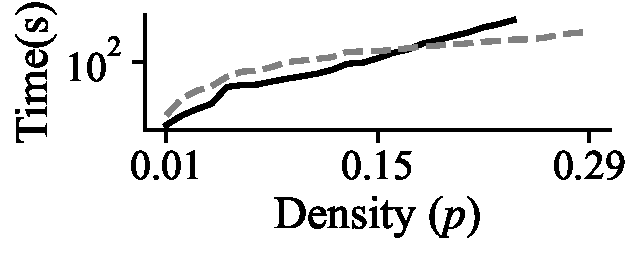
\includegraphics[width=\linewidth]{figure/runtime_r4_s5.pdf}
      \caption{r4 \\ s5}
    \end{subfigure}\hfill
    \begin{subfigure}[t]{0.24\linewidth}
      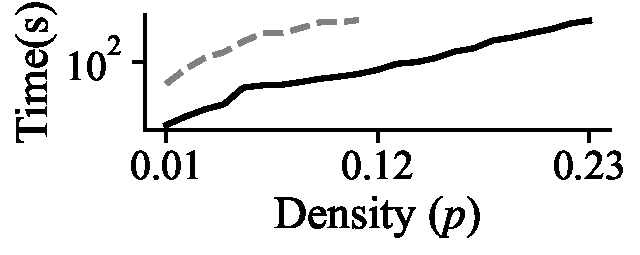
\includegraphics[width=\linewidth]{figure/runtime_r4_s6.pdf}
      \caption{r4 \\ s6}
    \end{subfigure}\hfill
    \begin{subfigure}[t]{0.24\linewidth}
      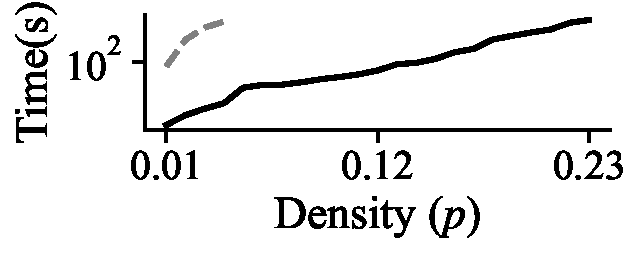
\includegraphics[width=\linewidth]{figure/runtime_r4_s7.pdf}
      \caption{r4 \\ s7}
    \end{subfigure}\hfill
    \begin{subfigure}[t]{0.24\linewidth}
      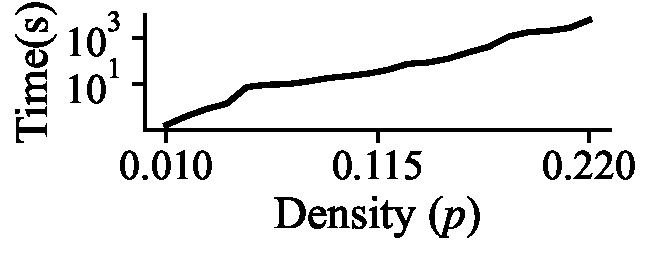
\includegraphics[width=\linewidth]{figure/runtime_r4_s8.pdf}
      \caption{r4 \\ s8}
    \end{subfigure}\hfill
    \begin{subfigure}[t]{0.24\linewidth}
      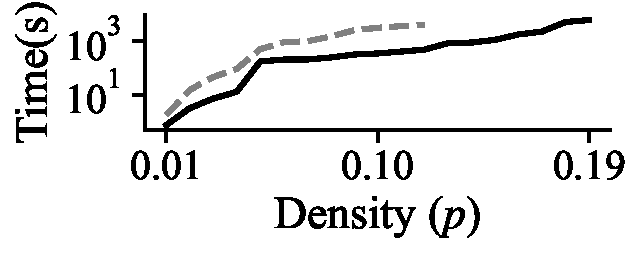
\includegraphics[width=\linewidth]{figure/runtime_r5_s6.pdf}
      \caption{r5 \\ s6}
    \end{subfigure}\hfill
    \begin{subfigure}[t]{0.24\linewidth}
      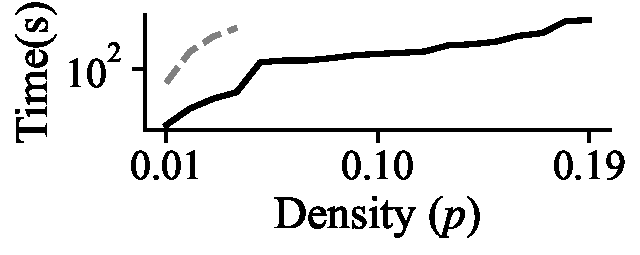
\includegraphics[width=\linewidth]{figure/runtime_r5_s7.pdf}
      \caption{r5 \\ s7}
    \end{subfigure}\hfill
    \begin{subfigure}[t]{0.24\linewidth}
      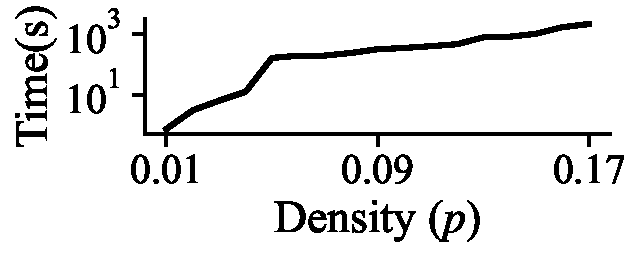
\includegraphics[width=\linewidth]{figure/runtime_r5_s8.pdf}
      \caption{r5 \\ s8}
    \end{subfigure}\hfill
    \begin{subfigure}[t]{0.24\linewidth}
      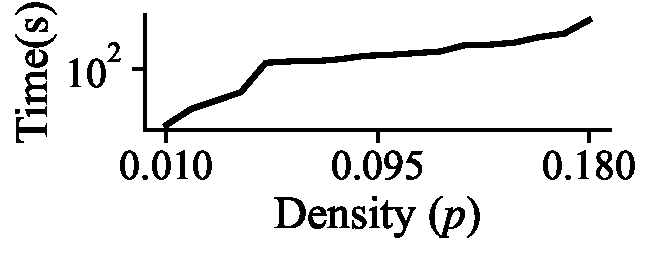
\includegraphics[width=\linewidth]{figure/runtime_r5_s9.pdf}
      \caption{r5 \\ s9}
    \end{subfigure}
  \end{minipage}
  
  

        \begin{minipage}[c]{0.02\textwidth}
    \centering
        % \raisebox{3em}{\rotatebox{90}{\tiny \textbf{Memory (Mb)}}}
  \end{minipage}  \hfill
  \begin{minipage}[c]{1\textwidth}
    \centering
    \begin{subfigure}[t]{0.24\linewidth}
      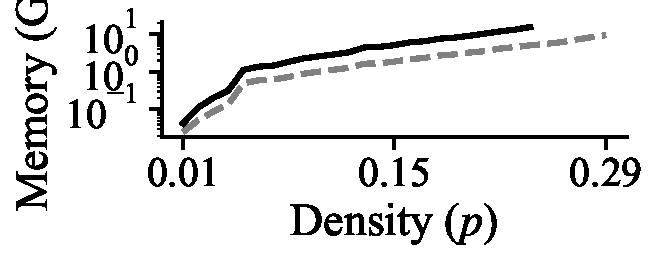
\includegraphics[width=\linewidth]{figure/memory_r4_s5.pdf}
      \caption{r4 \\ s5}
    \end{subfigure}\hfill
    \begin{subfigure}[t]{0.24\linewidth}
      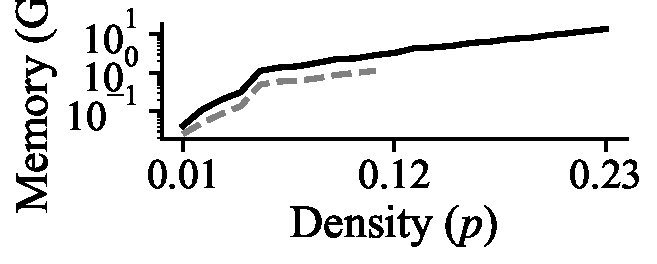
\includegraphics[width=\linewidth]{figure/memory_r4_s6.pdf}`'
      \caption{r4 \\ s6}
    \end{subfigure}\hfill
    \begin{subfigure}[t]{0.24\linewidth}
      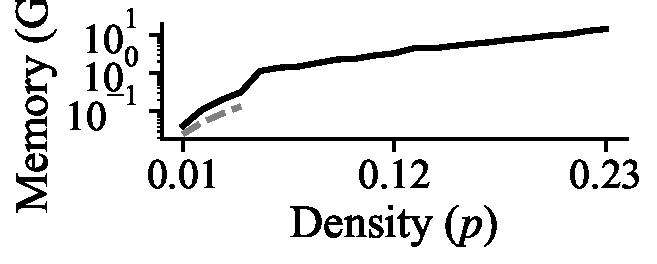
\includegraphics[width=\linewidth]{figure/memory_r4_s7.pdf}
      \caption{r4 \\ s7}
    \end{subfigure}\hfill
    \begin{subfigure}[t]{0.24\linewidth}
      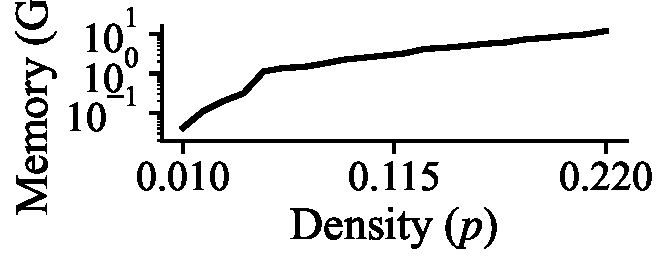
\includegraphics[width=\linewidth]{figure/memory_r4_s8.pdf}
      \caption{r4 \\ s8}
    \end{subfigure}\hfill
    \begin{subfigure}[t]{0.24\linewidth}
      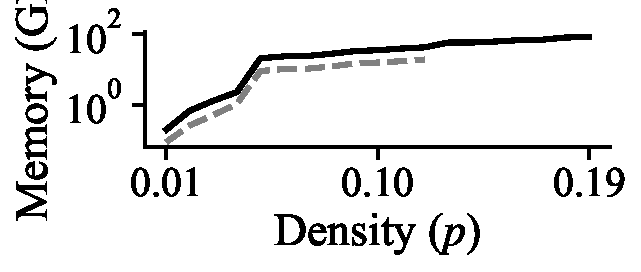
\includegraphics[width=\linewidth]{figure/memory_r5_s6.pdf}
      \caption{r5 \\ s6}
    \end{subfigure}\hfill
    \begin{subfigure}[t]{0.24\linewidth}
      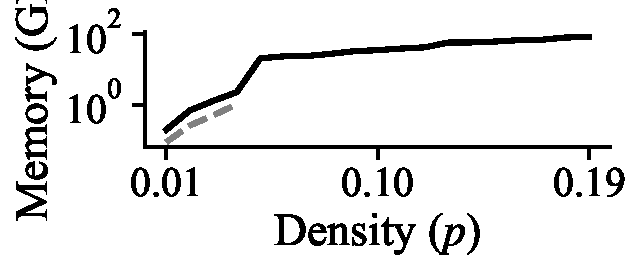
\includegraphics[width=\linewidth]{figure/memory_r5_s7.pdf}
      \caption{r5 \\ s7}
    \end{subfigure}\hfill
    \begin{subfigure}[t]{0.24\linewidth}
      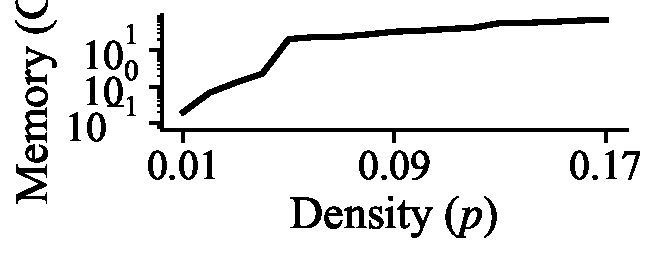
\includegraphics[width=\linewidth]{figure/memory_r5_s8.pdf}
      \caption{r5 \\ s8}
    \end{subfigure}\hfill
    \begin{subfigure}[t]{0.24\linewidth}
      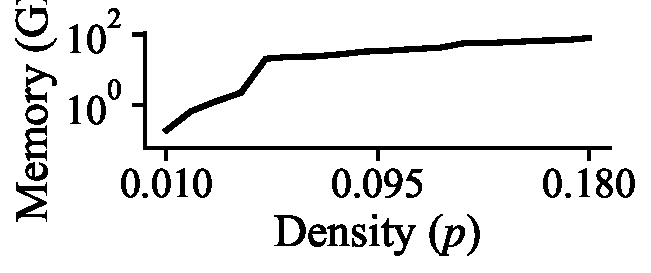
\includegraphics[width=\linewidth]{figure/memory_r5_s9.pdf}
      \caption{r5 \\ s9}
    \end{subfigure}
    
  \end{minipage}

  
  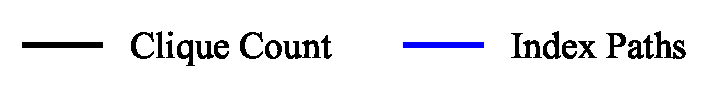
\includegraphics[width=0.4\textwidth]{figure/legend_leaf_clique.pdf}
  

  % \begin{minipage}[c]{0.02\textwidth}
  %   \centering
  %   % \raisebox{3em}{\rotatebox{90}{\tiny \textbf{Count}}}
  % \end{minipage}  \hfill
  \begin{minipage}[c]{1\textwidth}
    \centering
    \begin{subfigure}[t]{0.24\linewidth}
      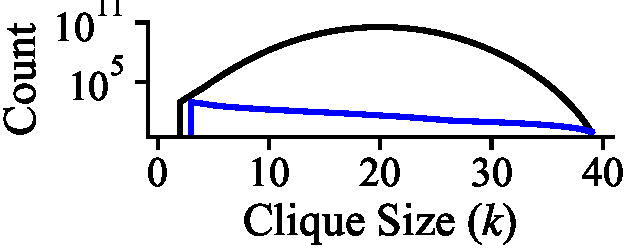
\includegraphics[width=\linewidth]{figure/snapshot_p0.01.pdf}
      \caption{p=0.01}
    \end{subfigure}\hfill
    \begin{subfigure}[t]{0.24\linewidth}
      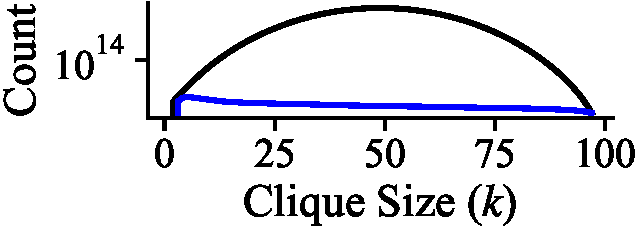
\includegraphics[width=\linewidth]{figure/snapshot_p0.06.pdf}
      \caption{p=0.06}
    \end{subfigure}\hfill
    \begin{subfigure}[t]{0.24\linewidth}
      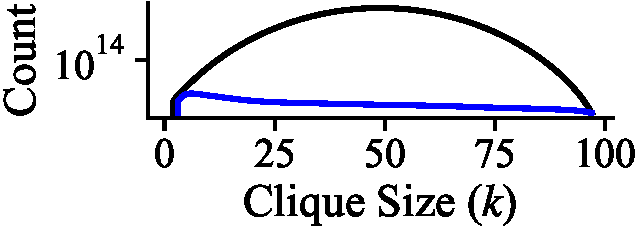
\includegraphics[width=\linewidth]{figure/snapshot_p0.11.pdf}
      \caption{p=0.11}
    \end{subfigure}\hfill
    \begin{subfigure}[t]{0.24 \linewidth}
      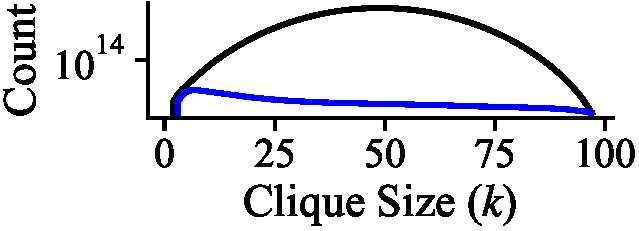
\includegraphics[width=\linewidth]{figure/snapshot_p0.16.pdf}
      \caption{p=0.16}
    \end{subfigure}\hfill
    \begin{subfigure}[t]{0.24\linewidth}
      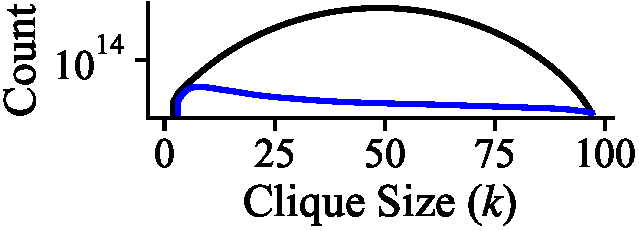
\includegraphics[width=\linewidth]{figure/snapshot_p0.22.pdf}
      \caption{p=0.22}
    \end{subfigure}\hfill
    \begin{subfigure}[t]{0.24\linewidth}
      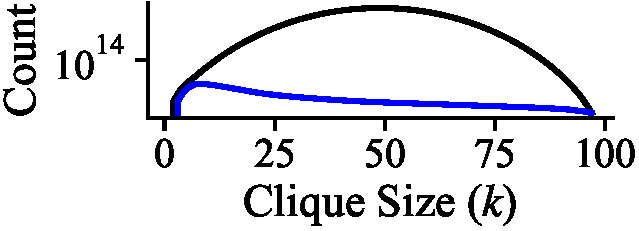
\includegraphics[width=\linewidth]{figure/snapshot_p0.27.pdf}
      \caption{p=0.27}
    \end{subfigure}\hfill
    \begin{subfigure}[t]{0.24\linewidth}
      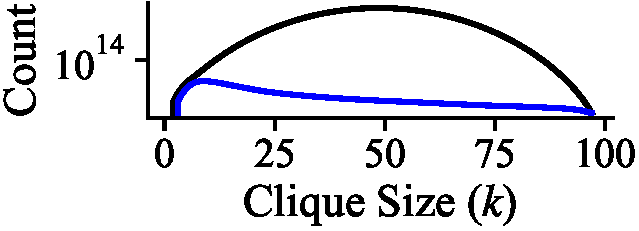
\includegraphics[width=\linewidth]{figure/snapshot_p0.32.pdf}
      \caption{p=0.32}
    \end{subfigure}\hfill
    \begin{subfigure}[t]{0.24\linewidth}
      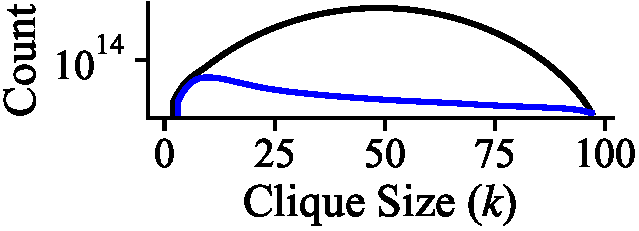
\includegraphics[width=\linewidth]{figure/snapshot_p0.38.pdf}
      \caption{p=0.38}
    \end{subfigure}
  \end{minipage}

  \caption{Comprehensive Stress Test Analysis. 
  \textbf{(a-h)} Runtime comparison across various $(r,s)$ pairs; 
  \textbf{(i-p)} Memory usage comparison corresponding to the top row; 
  \textbf{(q-x)} Leaf clique counts across varying densities ($p$).
  }
  \label{fig:stress_test_combined}
  
\end{figure}
